
\documentclass{article} % For LaTeX2e
\usepackage{iclr2021_conference,times}

% Optional math commands from https://github.com/goodfeli/dlbook_notation.
%%%%% NEW MATH DEFINITIONS %%%%%

\usepackage{amsmath,amsfonts,bm}

% Mark sections of captions for referring to divisions of figures
\newcommand{\figleft}{{\em (Left)}}
\newcommand{\figcenter}{{\em (Center)}}
\newcommand{\figright}{{\em (Right)}}
\newcommand{\figtop}{{\em (Top)}}
\newcommand{\figbottom}{{\em (Bottom)}}
\newcommand{\captiona}{{\em (a)}}
\newcommand{\captionb}{{\em (b)}}
\newcommand{\captionc}{{\em (c)}}
\newcommand{\captiond}{{\em (d)}}

% Highlight a newly defined term
\newcommand{\newterm}[1]{{\bf #1}}


% Figure reference, lower-case.
\def\figref#1{figure~\ref{#1}}
% Figure reference, capital. For start of sentence
\def\Figref#1{Figure~\ref{#1}}
\def\twofigref#1#2{figures \ref{#1} and \ref{#2}}
\def\quadfigref#1#2#3#4{figures \ref{#1}, \ref{#2}, \ref{#3} and \ref{#4}}
% Section reference, lower-case.
\def\secref#1{section~\ref{#1}}
% Section reference, capital.
\def\Secref#1{Section~\ref{#1}}
% Reference to two sections.
\def\twosecrefs#1#2{sections \ref{#1} and \ref{#2}}
% Reference to three sections.
\def\secrefs#1#2#3{sections \ref{#1}, \ref{#2} and \ref{#3}}
% Reference to an equation, lower-case.
\def\eqref#1{equation~\ref{#1}}
% Reference to an equation, upper case
\def\Eqref#1{Equation~\ref{#1}}
% A raw reference to an equation---avoid using if possible
\def\plaineqref#1{\ref{#1}}
% Reference to a chapter, lower-case.
\def\chapref#1{chapter~\ref{#1}}
% Reference to an equation, upper case.
\def\Chapref#1{Chapter~\ref{#1}}
% Reference to a range of chapters
\def\rangechapref#1#2{chapters\ref{#1}--\ref{#2}}
% Reference to an algorithm, lower-case.
\def\algref#1{algorithm~\ref{#1}}
% Reference to an algorithm, upper case.
\def\Algref#1{Algorithm~\ref{#1}}
\def\twoalgref#1#2{algorithms \ref{#1} and \ref{#2}}
\def\Twoalgref#1#2{Algorithms \ref{#1} and \ref{#2}}
% Reference to a part, lower case
\def\partref#1{part~\ref{#1}}
% Reference to a part, upper case
\def\Partref#1{Part~\ref{#1}}
\def\twopartref#1#2{parts \ref{#1} and \ref{#2}}

\def\ceil#1{\lceil #1 \rceil}
\def\floor#1{\lfloor #1 \rfloor}
\def\1{\bm{1}}
\newcommand{\train}{\mathcal{D}}
\newcommand{\valid}{\mathcal{D_{\mathrm{valid}}}}
\newcommand{\test}{\mathcal{D_{\mathrm{test}}}}

\def\eps{{\epsilon}}


% Random variables
\def\reta{{\textnormal{$\eta$}}}
\def\ra{{\textnormal{a}}}
\def\rb{{\textnormal{b}}}
\def\rc{{\textnormal{c}}}
\def\rd{{\textnormal{d}}}
\def\re{{\textnormal{e}}}
\def\rf{{\textnormal{f}}}
\def\rg{{\textnormal{g}}}
\def\rh{{\textnormal{h}}}
\def\ri{{\textnormal{i}}}
\def\rj{{\textnormal{j}}}
\def\rk{{\textnormal{k}}}
\def\rl{{\textnormal{l}}}
% rm is already a command, just don't name any random variables m
\def\rn{{\textnormal{n}}}
\def\ro{{\textnormal{o}}}
\def\rp{{\textnormal{p}}}
\def\rq{{\textnormal{q}}}
\def\rr{{\textnormal{r}}}
\def\rs{{\textnormal{s}}}
\def\rt{{\textnormal{t}}}
\def\ru{{\textnormal{u}}}
\def\rv{{\textnormal{v}}}
\def\rw{{\textnormal{w}}}
\def\rx{{\textnormal{x}}}
\def\ry{{\textnormal{y}}}
\def\rz{{\textnormal{z}}}

% Random vectors
\def\rvepsilon{{\mathbf{\epsilon}}}
\def\rvtheta{{\mathbf{\theta}}}
\def\rva{{\mathbf{a}}}
\def\rvb{{\mathbf{b}}}
\def\rvc{{\mathbf{c}}}
\def\rvd{{\mathbf{d}}}
\def\rve{{\mathbf{e}}}
\def\rvf{{\mathbf{f}}}
\def\rvg{{\mathbf{g}}}
\def\rvh{{\mathbf{h}}}
\def\rvu{{\mathbf{i}}}
\def\rvj{{\mathbf{j}}}
\def\rvk{{\mathbf{k}}}
\def\rvl{{\mathbf{l}}}
\def\rvm{{\mathbf{m}}}
\def\rvn{{\mathbf{n}}}
\def\rvo{{\mathbf{o}}}
\def\rvp{{\mathbf{p}}}
\def\rvq{{\mathbf{q}}}
\def\rvr{{\mathbf{r}}}
\def\rvs{{\mathbf{s}}}
\def\rvt{{\mathbf{t}}}
\def\rvu{{\mathbf{u}}}
\def\rvv{{\mathbf{v}}}
\def\rvw{{\mathbf{w}}}
\def\rvx{{\mathbf{x}}}
\def\rvy{{\mathbf{y}}}
\def\rvz{{\mathbf{z}}}

% Elements of random vectors
\def\erva{{\textnormal{a}}}
\def\ervb{{\textnormal{b}}}
\def\ervc{{\textnormal{c}}}
\def\ervd{{\textnormal{d}}}
\def\erve{{\textnormal{e}}}
\def\ervf{{\textnormal{f}}}
\def\ervg{{\textnormal{g}}}
\def\ervh{{\textnormal{h}}}
\def\ervi{{\textnormal{i}}}
\def\ervj{{\textnormal{j}}}
\def\ervk{{\textnormal{k}}}
\def\ervl{{\textnormal{l}}}
\def\ervm{{\textnormal{m}}}
\def\ervn{{\textnormal{n}}}
\def\ervo{{\textnormal{o}}}
\def\ervp{{\textnormal{p}}}
\def\ervq{{\textnormal{q}}}
\def\ervr{{\textnormal{r}}}
\def\ervs{{\textnormal{s}}}
\def\ervt{{\textnormal{t}}}
\def\ervu{{\textnormal{u}}}
\def\ervv{{\textnormal{v}}}
\def\ervw{{\textnormal{w}}}
\def\ervx{{\textnormal{x}}}
\def\ervy{{\textnormal{y}}}
\def\ervz{{\textnormal{z}}}

% Random matrices
\def\rmA{{\mathbf{A}}}
\def\rmB{{\mathbf{B}}}
\def\rmC{{\mathbf{C}}}
\def\rmD{{\mathbf{D}}}
\def\rmE{{\mathbf{E}}}
\def\rmF{{\mathbf{F}}}
\def\rmG{{\mathbf{G}}}
\def\rmH{{\mathbf{H}}}
\def\rmI{{\mathbf{I}}}
\def\rmJ{{\mathbf{J}}}
\def\rmK{{\mathbf{K}}}
\def\rmL{{\mathbf{L}}}
\def\rmM{{\mathbf{M}}}
\def\rmN{{\mathbf{N}}}
\def\rmO{{\mathbf{O}}}
\def\rmP{{\mathbf{P}}}
\def\rmQ{{\mathbf{Q}}}
\def\rmR{{\mathbf{R}}}
\def\rmS{{\mathbf{S}}}
\def\rmT{{\mathbf{T}}}
\def\rmU{{\mathbf{U}}}
\def\rmV{{\mathbf{V}}}
\def\rmW{{\mathbf{W}}}
\def\rmX{{\mathbf{X}}}
\def\rmY{{\mathbf{Y}}}
\def\rmZ{{\mathbf{Z}}}

% Elements of random matrices
\def\ermA{{\textnormal{A}}}
\def\ermB{{\textnormal{B}}}
\def\ermC{{\textnormal{C}}}
\def\ermD{{\textnormal{D}}}
\def\ermE{{\textnormal{E}}}
\def\ermF{{\textnormal{F}}}
\def\ermG{{\textnormal{G}}}
\def\ermH{{\textnormal{H}}}
\def\ermI{{\textnormal{I}}}
\def\ermJ{{\textnormal{J}}}
\def\ermK{{\textnormal{K}}}
\def\ermL{{\textnormal{L}}}
\def\ermM{{\textnormal{M}}}
\def\ermN{{\textnormal{N}}}
\def\ermO{{\textnormal{O}}}
\def\ermP{{\textnormal{P}}}
\def\ermQ{{\textnormal{Q}}}
\def\ermR{{\textnormal{R}}}
\def\ermS{{\textnormal{S}}}
\def\ermT{{\textnormal{T}}}
\def\ermU{{\textnormal{U}}}
\def\ermV{{\textnormal{V}}}
\def\ermW{{\textnormal{W}}}
\def\ermX{{\textnormal{X}}}
\def\ermY{{\textnormal{Y}}}
\def\ermZ{{\textnormal{Z}}}

% Vectors
\def\vzero{{\bm{0}}}
\def\vone{{\bm{1}}}
\def\vmu{{\bm{\mu}}}
\def\vtheta{{\bm{\theta}}}
\def\va{{\bm{a}}}
\def\vb{{\bm{b}}}
\def\vc{{\bm{c}}}
\def\vd{{\bm{d}}}
\def\ve{{\bm{e}}}
\def\vf{{\bm{f}}}
\def\vg{{\bm{g}}}
\def\vh{{\bm{h}}}
\def\vi{{\bm{i}}}
\def\vj{{\bm{j}}}
\def\vk{{\bm{k}}}
\def\vl{{\bm{l}}}
\def\vm{{\bm{m}}}
\def\vn{{\bm{n}}}
\def\vo{{\bm{o}}}
\def\vp{{\bm{p}}}
\def\vq{{\bm{q}}}
\def\vr{{\bm{r}}}
\def\vs{{\bm{s}}}
\def\vt{{\bm{t}}}
\def\vu{{\bm{u}}}
\def\vv{{\bm{v}}}
\def\vw{{\bm{w}}}
\def\vx{{\bm{x}}}
\def\vy{{\bm{y}}}
\def\vz{{\bm{z}}}

% Elements of vectors
\def\evalpha{{\alpha}}
\def\evbeta{{\beta}}
\def\evepsilon{{\epsilon}}
\def\evlambda{{\lambda}}
\def\evomega{{\omega}}
\def\evmu{{\mu}}
\def\evpsi{{\psi}}
\def\evsigma{{\sigma}}
\def\evtheta{{\theta}}
\def\eva{{a}}
\def\evb{{b}}
\def\evc{{c}}
\def\evd{{d}}
\def\eve{{e}}
\def\evf{{f}}
\def\evg{{g}}
\def\evh{{h}}
\def\evi{{i}}
\def\evj{{j}}
\def\evk{{k}}
\def\evl{{l}}
\def\evm{{m}}
\def\evn{{n}}
\def\evo{{o}}
\def\evp{{p}}
\def\evq{{q}}
\def\evr{{r}}
\def\evs{{s}}
\def\evt{{t}}
\def\evu{{u}}
\def\evv{{v}}
\def\evw{{w}}
\def\evx{{x}}
\def\evy{{y}}
\def\evz{{z}}

% Matrix
\def\mA{{\bm{A}}}
\def\mB{{\bm{B}}}
\def\mC{{\bm{C}}}
\def\mD{{\bm{D}}}
\def\mE{{\bm{E}}}
\def\mF{{\bm{F}}}
\def\mG{{\bm{G}}}
\def\mH{{\bm{H}}}
\def\mI{{\bm{I}}}
\def\mJ{{\bm{J}}}
\def\mK{{\bm{K}}}
\def\mL{{\bm{L}}}
\def\mM{{\bm{M}}}
\def\mN{{\bm{N}}}
\def\mO{{\bm{O}}}
\def\mP{{\bm{P}}}
\def\mQ{{\bm{Q}}}
\def\mR{{\bm{R}}}
\def\mS{{\bm{S}}}
\def\mT{{\bm{T}}}
\def\mU{{\bm{U}}}
\def\mV{{\bm{V}}}
\def\mW{{\bm{W}}}
\def\mX{{\bm{X}}}
\def\mY{{\bm{Y}}}
\def\mZ{{\bm{Z}}}
\def\mBeta{{\bm{\beta}}}
\def\mPhi{{\bm{\Phi}}}
\def\mLambda{{\bm{\Lambda}}}
\def\mSigma{{\bm{\Sigma}}}

% Tensor
\DeclareMathAlphabet{\mathsfit}{\encodingdefault}{\sfdefault}{m}{sl}
\SetMathAlphabet{\mathsfit}{bold}{\encodingdefault}{\sfdefault}{bx}{n}
\newcommand{\tens}[1]{\bm{\mathsfit{#1}}}
\def\tA{{\tens{A}}}
\def\tB{{\tens{B}}}
\def\tC{{\tens{C}}}
\def\tD{{\tens{D}}}
\def\tE{{\tens{E}}}
\def\tF{{\tens{F}}}
\def\tG{{\tens{G}}}
\def\tH{{\tens{H}}}
\def\tI{{\tens{I}}}
\def\tJ{{\tens{J}}}
\def\tK{{\tens{K}}}
\def\tL{{\tens{L}}}
\def\tM{{\tens{M}}}
\def\tN{{\tens{N}}}
\def\tO{{\tens{O}}}
\def\tP{{\tens{P}}}
\def\tQ{{\tens{Q}}}
\def\tR{{\tens{R}}}
\def\tS{{\tens{S}}}
\def\tT{{\tens{T}}}
\def\tU{{\tens{U}}}
\def\tV{{\tens{V}}}
\def\tW{{\tens{W}}}
\def\tX{{\tens{X}}}
\def\tY{{\tens{Y}}}
\def\tZ{{\tens{Z}}}


% Graph
\def\gA{{\mathcal{A}}}
\def\gB{{\mathcal{B}}}
\def\gC{{\mathcal{C}}}
\def\gD{{\mathcal{D}}}
\def\gE{{\mathcal{E}}}
\def\gF{{\mathcal{F}}}
\def\gG{{\mathcal{G}}}
\def\gH{{\mathcal{H}}}
\def\gI{{\mathcal{I}}}
\def\gJ{{\mathcal{J}}}
\def\gK{{\mathcal{K}}}
\def\gL{{\mathcal{L}}}
\def\gM{{\mathcal{M}}}
\def\gN{{\mathcal{N}}}
\def\gO{{\mathcal{O}}}
\def\gP{{\mathcal{P}}}
\def\gQ{{\mathcal{Q}}}
\def\gR{{\mathcal{R}}}
\def\gS{{\mathcal{S}}}
\def\gT{{\mathcal{T}}}
\def\gU{{\mathcal{U}}}
\def\gV{{\mathcal{V}}}
\def\gW{{\mathcal{W}}}
\def\gX{{\mathcal{X}}}
\def\gY{{\mathcal{Y}}}
\def\gZ{{\mathcal{Z}}}

% Sets
\def\sA{{\mathbb{A}}}
\def\sB{{\mathbb{B}}}
\def\sC{{\mathbb{C}}}
\def\sD{{\mathbb{D}}}
% Don't use a set called E, because this would be the same as our symbol
% for expectation.
\def\sF{{\mathbb{F}}}
\def\sG{{\mathbb{G}}}
\def\sH{{\mathbb{H}}}
\def\sI{{\mathbb{I}}}
\def\sJ{{\mathbb{J}}}
\def\sK{{\mathbb{K}}}
\def\sL{{\mathbb{L}}}
\def\sM{{\mathbb{M}}}
\def\sN{{\mathbb{N}}}
\def\sO{{\mathbb{O}}}
\def\sP{{\mathbb{P}}}
\def\sQ{{\mathbb{Q}}}
\def\sR{{\mathbb{R}}}
\def\sS{{\mathbb{S}}}
\def\sT{{\mathbb{T}}}
\def\sU{{\mathbb{U}}}
\def\sV{{\mathbb{V}}}
\def\sW{{\mathbb{W}}}
\def\sX{{\mathbb{X}}}
\def\sY{{\mathbb{Y}}}
\def\sZ{{\mathbb{Z}}}

% Entries of a matrix
\def\emLambda{{\Lambda}}
\def\emA{{A}}
\def\emB{{B}}
\def\emC{{C}}
\def\emD{{D}}
\def\emE{{E}}
\def\emF{{F}}
\def\emG{{G}}
\def\emH{{H}}
\def\emI{{I}}
\def\emJ{{J}}
\def\emK{{K}}
\def\emL{{L}}
\def\emM{{M}}
\def\emN{{N}}
\def\emO{{O}}
\def\emP{{P}}
\def\emQ{{Q}}
\def\emR{{R}}
\def\emS{{S}}
\def\emT{{T}}
\def\emU{{U}}
\def\emV{{V}}
\def\emW{{W}}
\def\emX{{X}}
\def\emY{{Y}}
\def\emZ{{Z}}
\def\emSigma{{\Sigma}}

% entries of a tensor
% Same font as tensor, without \bm wrapper
\newcommand{\etens}[1]{\mathsfit{#1}}
\def\etLambda{{\etens{\Lambda}}}
\def\etA{{\etens{A}}}
\def\etB{{\etens{B}}}
\def\etC{{\etens{C}}}
\def\etD{{\etens{D}}}
\def\etE{{\etens{E}}}
\def\etF{{\etens{F}}}
\def\etG{{\etens{G}}}
\def\etH{{\etens{H}}}
\def\etI{{\etens{I}}}
\def\etJ{{\etens{J}}}
\def\etK{{\etens{K}}}
\def\etL{{\etens{L}}}
\def\etM{{\etens{M}}}
\def\etN{{\etens{N}}}
\def\etO{{\etens{O}}}
\def\etP{{\etens{P}}}
\def\etQ{{\etens{Q}}}
\def\etR{{\etens{R}}}
\def\etS{{\etens{S}}}
\def\etT{{\etens{T}}}
\def\etU{{\etens{U}}}
\def\etV{{\etens{V}}}
\def\etW{{\etens{W}}}
\def\etX{{\etens{X}}}
\def\etY{{\etens{Y}}}
\def\etZ{{\etens{Z}}}

% The true underlying data generating distribution
\newcommand{\pdata}{p_{\rm{data}}}
% The empirical distribution defined by the training set
\newcommand{\ptrain}{\hat{p}_{\rm{data}}}
\newcommand{\Ptrain}{\hat{P}_{\rm{data}}}
% The model distribution
\newcommand{\pmodel}{p_{\rm{model}}}
\newcommand{\Pmodel}{P_{\rm{model}}}
\newcommand{\ptildemodel}{\tilde{p}_{\rm{model}}}
% Stochastic autoencoder distributions
\newcommand{\pencode}{p_{\rm{encoder}}}
\newcommand{\pdecode}{p_{\rm{decoder}}}
\newcommand{\precons}{p_{\rm{reconstruct}}}

\newcommand{\laplace}{\mathrm{Laplace}} % Laplace distribution

\newcommand{\E}{\mathbb{E}}
\newcommand{\Ls}{\mathcal{L}}
\newcommand{\R}{\mathbb{R}}
\newcommand{\emp}{\tilde{p}}
\newcommand{\lr}{\alpha}
\newcommand{\reg}{\lambda}
\newcommand{\rect}{\mathrm{rectifier}}
\newcommand{\softmax}{\mathrm{softmax}}
\newcommand{\sigmoid}{\sigma}
\newcommand{\softplus}{\zeta}
\newcommand{\KL}{D_{\mathrm{KL}}}
\newcommand{\Var}{\mathrm{Var}}
\newcommand{\standarderror}{\mathrm{SE}}
\newcommand{\Cov}{\mathrm{Cov}}
% Wolfram Mathworld says $L^2$ is for function spaces and $\ell^2$ is for vectors
% But then they seem to use $L^2$ for vectors throughout the site, and so does
% wikipedia.
\newcommand{\normlzero}{L^0}
\newcommand{\normlone}{L^1}
\newcommand{\normltwo}{L^2}
\newcommand{\normlp}{L^p}
\newcommand{\normmax}{L^\infty}

\newcommand{\parents}{Pa} % See usage in notation.tex. Chosen to match Daphne's book.

\DeclareMathOperator*{\argmax}{arg\,max}
\DeclareMathOperator*{\argmin}{arg\,min}

\DeclareMathOperator{\sign}{sign}
\DeclareMathOperator{\Tr}{Tr}
\let\ab\allowbreak


\usepackage{hyperref}
\usepackage{url}

\usepackage{float}
\usepackage{graphicx}
\usepackage{caption}
\usepackage{subcaption}


\title{Genmo Combo:\\
Bridging Mental Health, Genetics, and Clinical Trials with LLM and Sentiment Analysis
}

\author{Tingyu Liu\\ School of Computational Science and Engineering\\Georgia Tech\\ \\  \url{tliu479@gatech.edu} \\ \\ \href{https://github.com/taraliu23/Turmerik-MLE-Takehome}{GitHub Repository}}


\newcommand{\fix}{\marginpar{FIX}}
\newcommand{\new}{\marginpar{NEW}}

\iclrfinalcopy 
\begin{document}

\maketitle

\begin{abstract}
Patients with co-occurring mental health disorders and genetic conditions face significant challenges in accessing resources, navigating clinical trials, and receiving personalized care. This project addresses these gaps by developing a WebApp that integrates sentiment analysis and Retrieval-Augmented Generation (RAG) to provide trustworthy, contextually relevant information.

The study leverages subreddit discussions to analyze public sentiment and uses these insights to inform the design of an interactive Q&A chat interface and a static knowledge hub. The WebApp empowers users, especially those without a research background, to access curated resources and answers to their queries. Sentiment analysis revealed pervasive frustrations and gaps in existing support systems, emphasizing the need for patient-centered tools.The results demonstrate the potential of RAG-enhanced language models to minimize hallucinations and provide accurate responses, as validated through a 50-question simulated Q&A evaluation. While the current implementation focuses on foundational functionalities, future enhancements will include personalized recommendations, advanced clinical trial search, and robust privacy features.

This work highlights the transformative role of AI in bridging healthcare accessibility gaps, particularly for underserved populations. By combining advanced computational methods with patient-centric design, the project sets the stage for a comprehensive platform that addresses the unique needs of individuals with genetic-linked mental disorders.

\end{abstract}

\section{Problem Statement}

\subsection{Background}


Mental disorders, such as depression and anxiety, are caused by a compound influence of environmental and genetic factors \citep{alshaya2022depression}. All major psychiatric disorders have genetic risk factors, and genetic strategies are frequently employed to evaluate possible overlaps. 


For example, common genetics variation single nucleotide polymorphisms (SNPs) appeared more frequently in individuals with five prevalent mental disorders: autism spectrum disorder (ASD), attention deficit-hyperactivity disorder (ADHD), bipolar disorder, major depressive disorder, and schizophrenia \citep{Cross-Disorder}. 



\subsection{Problem Statement}

Patients with co-occuring genetic diseases and mental disorders experience a set of interconnected challenges, including healthcare inequity, social stigma, and privacy concerns.

They must navigate the diagnostic difficulties associated with both conditions, where genetic diseases with long and costly diagnostic process \citep{Breining_2018} and  mental  disorder with misdiagnosis issues. 

They are often excluded from mental health trials, further limiting their treatment options. Additionally, a significant proportion of mental disorder clinical trials exclude individuals with additional medical conditions. 

The limited treatment options for genetic conditions combined with barriers to accessing mental healthcare create a compound effect on their healthcare management, which could further lead to financial instability, creating a cyclical pattern of hardship.

These individuals also bear a double burden of social stigma and face discrimination \citep{Barriers}, leading to potential isolation, anxiety, and depression from both conditions along with physical symptoms of their genetic disease.

The use of Large Language Models (LLMs) in mental health care and genetic disease management depend on heavily user-genrerated prompts, and could be inherent biased. Hallucinations and inaccuries in answer would lead to serious consquence. Also, Large language models (LLMs) such as ChatGPT often refuse valid health-related queries due to overzealous ethical safeguards, leaving patients without critical information \citep{Guo_2024}.

\subsection{Motivation}


This project aim to address the needs of patients with co-occurring mental health and genetic disorders by providing self-help resources, facilitating access in clinical trials and improving knowledge accessibility.

Providing Self-Help Resources: Empowering patients to take proactive steps in managing their conditions.

Facilitating Access to Clinical Trials: Helping patients identify appropriate clinical trials tailored to their unique genetic and mental health profiles.

Improving Accessibility: Developing tools that cater to patients without a research or medical background, thereby bridging the knowledge gap.


% to cite: use \citet{Bengio+chapter2007} or \citep{Hinton06}

\section{Literature Survey}

\subsection{Applications of LLMs in mental health care}

Diagnosis: LLMs assist in identifying mental health conditions by analyzing patient data and clinical notes.

Therapy: They support therapeutic interventions through chatbots and virtual agents, providing cognitive behavioral therapy and other therapeutic modalities.

Patient Engagement: LLMs enhance patient engagement by facilitating communication and providing psycho-education.

\subsection{Models for LLMs in mental disorder-genetics disease}

Before 2023, the most common LLMs used for mental health disease detection are GPT-3 (\citet{10079554}, \citet{10.1145/3544549.3585614}) and BERT(\citet{Diniz_Fontenele_de2022},\citet{Tanana_Soma_Kuo_Bertagnolli_Dembe_Pace_Srikumar_Atkins_Imel_2021}). In 2023 and 2024, the LLMs become diverserse, including ChatGPT 4.0\citep{BLEASE2024115724}, bing AI, Claude, Bard\citep{Elyoseph_Levkovich_Shinan-Altman_2024}, and open source models like LlaA-7B, ChatGLM-6b\citet{10263217}.

\subsection{Current Challenges for LLM in mental disorder and genetics disease}


LLMs have been tested and, to a limited degree, implemented in a variety of medical applications. There are some studies showing that LLMs perform better than human physicians in terms of the responses that patients prefer. However, there is ample evidence of LLMs' shortcomings in mental health counseling\citet{chung2023challengeslargelanguagemodels}.

Challenges of LLMs for mental health and genetics diesease counseling include model hellucination, interpretebility of AI, electronics health records, bias

Ethical worries include the lack of a well-defined, industry-standard ethical structure; issues related to data privacy; and the possibility that patients and doctors will rely too much on LLMs, risking conventional medical procedures. 



\subsection{Case Study}


A notable example is Boosting GPT Models for Genomics Analysis [9], which demonstrates the application of Retrieval-Augmented Generation (RAG) for generating trusted genetic variant annotations and interpretations. While promising, this approach does not integrate patient-specific needs or mental health aspects, highlighting the gap this study aims to address.


Existing tools primarily focus on leveraging clinical databases, but they lack the ability to address key issues, such as patient sentiments, tailored resources, and open source implementation.

Patient Needs and Sentiments: Current systems do not consider the emotional and informational needs of patients, particularly those with genetic-linked mental disorders.

Tailored Resources: There is an absence of resources specifically designed for individuals with co-occurring genetic and mental health conditions.

Open-Source Implementation: Most existing solutions are proprietary, limiting accessibility and scalability.



\section{Method}

\begin{figure}[h]
\begin{center}
%\framebox[4.0in]{$\;$}
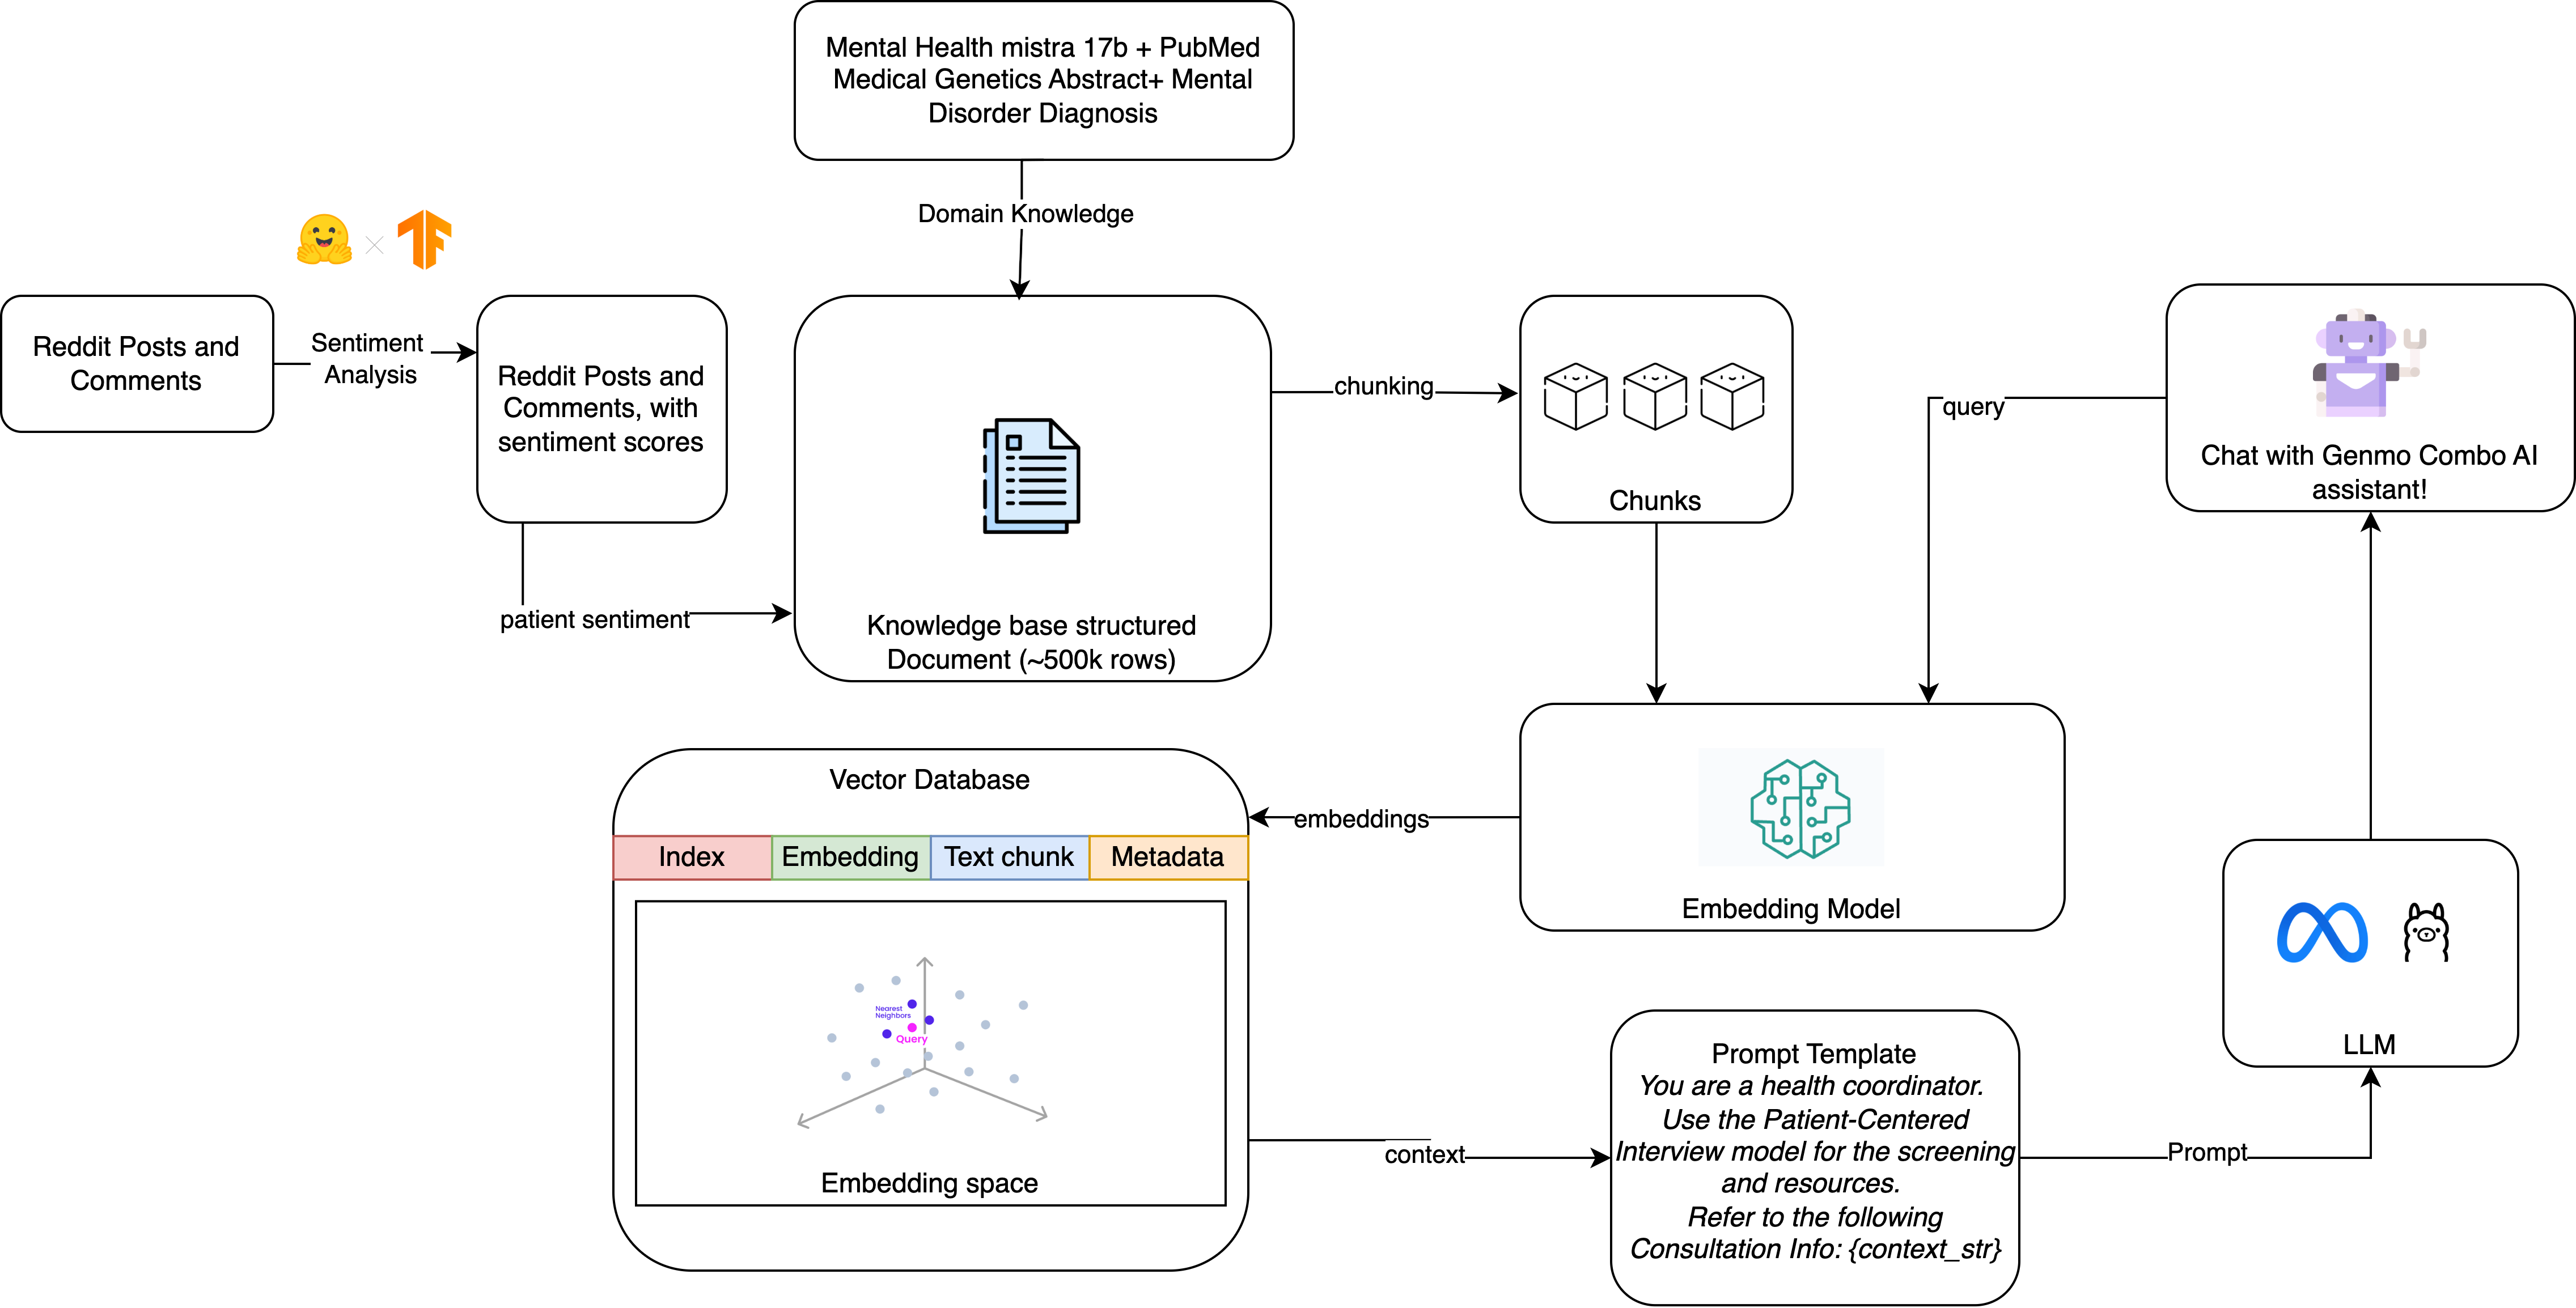
\includegraphics[width=\textwidth]{fig/workflow.png}
% \fbox{\rule[-.5cm]{0cm}{4cm} \rule[-.5cm]{4cm}{0cm}}
\end{center}
\caption{Workflow}
\end{figure}

\subsection{Retrieval-Augmented Generation (RAG)}

This project uses Retrieval-Augmented Generation (RAG) to improve the accuracy and reliability of LLM (Llama-2-7B-Chat\citet{touvron2023llama2openfoundation}) outputs while addressing patient-specific needs. 

Llama 2 is a collection of pretrained and fine-tuned generative text models ranging in scale from 7 billion to 70 billion parameters.

The method includes:

Sentiment Analysis with Transformers: Using state-of-the-art models to analyze patient sentiment and identify emotional or informational gaps.

RAG Implementation with Llama2-cpp: Integrating RAG to enhance retrieval capabilities, ensuring that LLM outputs are grounded in relevant, trusted data.

Fine-Tuning and Hallucination Control:
Fine-tuning LLMs with domain-specific data minimizes the likelihood of generating hallucinated information.

Keeping the LLM fixed while employing retrieval ensures the integrity and reliability of generated content.

By combining sentiment analysis with RAG, this approach prioritizes patient needs while maintaining control over the accuracy and relevance of the model's outputs.

\subsection{Data}



\section{Result and Conclusion}

The system was evaluated through a 50-question simulated Q&A comparison, with responses assessed by human reviewers and ChatGPT-4.0 for:

Helpfulness: Assessing the relevance and accuracy of the response.
Structural Compliance: Evaluating whether the response adhered to a logical and user-friendly structure.
Task Completeness: Ensuring that the response fully addressed the user’s query.

\subsection{sentiment analysis}

\subsection{Model Evaluation}
50 simulated Q\&A binary comparison:
Responses were evaluated and tagged by human and chatGPT 4o reviewers for helpfulness.
structural compliance
task completeness

\subsection{WebApp}

A web-based tool was developed to:

Provide patients with access to curated self-help resources and clinical trials.
Offer personalized recommendations based on sentiment and query analysis.
Ensure security and privacy, addressing concerns raised by the use of commercial LLMs.

Implemented Functionalities
The current implementation of the WebApp focuses on two core features to address immediate patient needs:

Interactive Q&A Chat Interface:

Functionality: A chatbot-style interface powered by a Retrieval-Augmented Generation (RAG)-enhanced LLM.
Description:
Patients can ask questions about mental health and genetic disorders, and the system provides informative responses based on trusted resources.
The RAG component minimizes hallucinations by grounding responses in retrieved data.
Current Scope: The interface supports single-turn and basic multi-turn queries for general questions.
Resource Knowledge Cards:

Functionality: A static knowledge hub providing curated educational content.
Description:
Knowledge cards contain general information on topics such as clinical trial participation, genetic counseling, and mental health management.
Designed to help users without a research background understand complex topics.
Limitations
The chatbot does not yet provide personalized responses based on patient sentiment or medical history.
The knowledge hub is static and lacks advanced filtering or search functionality.

\subsection{Future Work}

To expand the WebApp's capabilities and improve patient support, several additional features are planned for future development:

Personalized Resource Recommendations:

Use sentiment analysis and patient-specific data to provide tailored clinical trial suggestions and self-help resources.
Integrate dynamic filtering based on user preferences, eligibility criteria, and geographic location.
Advanced Clinical Trial Search:

Enable patients to search for trials using advanced filters, such as genetic markers, trial phases, and eligibility requirements.
Include visual summaries of trial information for improved usability.
Privacy and Security Enhancements:

Implement end-to-end encryption and strict anonymization protocols for user queries.
Ensure compliance with HIPAA and GDPR to address privacy concerns.
Educational Resource Expansion:

Develop multilingual content and interactive tutorials to cater to a global and diverse audience.
Add a recommendation system for related knowledge cards based on user queries.
Feedback Mechanism:

Allow users to provide feedback on chatbot responses and knowledge cards.
Use feedback to iteratively improve the model and resource database.
Multi-Language Support:

Integrate translation models to provide responses in multiple languages, making the app accessible to non-English-speaking users.
Accessibility Features:

Add features such as screen-reader compatibility, high-contrast themes, and keyboard navigation to ensure inclusivity.
Integration with External Systems:

Develop APIs for interoperability with healthcare provider systems, genetic testing platforms, and patient support networks.
Analytics Dashboard:

Create a dashboard for administrators to monitor usage metrics, system performance, and user feedback trends.
Use analytics to identify gaps and prioritize updates.





\section{Conclusion}

This project addresses a critical gap in the intersection of mental health and genetics by developing tools that empower patients to access relevant resources and support. By leveraging advanced techniques such as sentiment analysis and Retrieval-Augmented Generation (RAG), the study provides innovative solutions to assist individuals with genetic-linked mental disorders.

The project achieved significant milestones, including the implementation of an interactive Q&A chat interface and a static knowledge hub, which collectively form the foundation of the WebApp. These features cater to patients' immediate needs by delivering trustworthy information in an accessible format, especially for those lacking a research background.

The sentiment analysis component highlighted the prevailing frustrations and hopes of patients, offering valuable insights into user needs. Evaluations through simulated Q&A demonstrated the potential of RAG-enhanced LLMs to provide reliable, contextually relevant responses while minimizing hallucinations. The methodologies and findings underscore the importance of combining machine learning advancements with patient-centric design.

Key Contributions
Developed a WebApp prototype that integrates RAG-enhanced LLMs and knowledge cards to improve patient access to mental health and genetic disorder resources.
Conducted a comprehensive sentiment analysis of online discussions, revealing critical gaps in current systems and user pain points.
Established a scalable framework for future enhancements, including personalization, multi-language support, and robust privacy features.
Future Implications
This study lays the groundwork for creating a comprehensive platform that not only supports patients in navigating clinical trials but also addresses their broader emotional and informational needs. Future work will focus on implementing dynamic personalization, expanding accessibility, and fostering trust through enhanced privacy and security protocols.

Final Remarks
By integrating cutting-edge computational methods with an understanding of patient challenges, this project contributes to the evolving field of digital health. It demonstrates the potential for technology to bridge the gaps in healthcare access and provide meaningful support to underserved populations. Continued collaboration and iterative improvements will ensure that the platform becomes an indispensable resource for patients with genetic-linked mental disorders, ultimately advancing personalized care and patient empowerment.



% \begin{verbatim}
%    \usepackage[dvips]{graphicx} ...
%    \includegraphics[width=0.8\linewidth]{myfile.eps}
% \end{verbatim}
or % Apr 2009 addition

\subsubsection*{Author Contributions}
Tingyu Liu: project management, LLM RAG, full-stack devlopment, data engineering, report and presentation.

\bibliography{iclr2021_conference}
\bibliographystyle{iclr2021_conference}

\appendix
\section{Appendix}
You may include other additional sections here.

\end{document}
